\begin{frame}{Zugfolge f�r $n=6$ und $k=4$}
\only<1>{
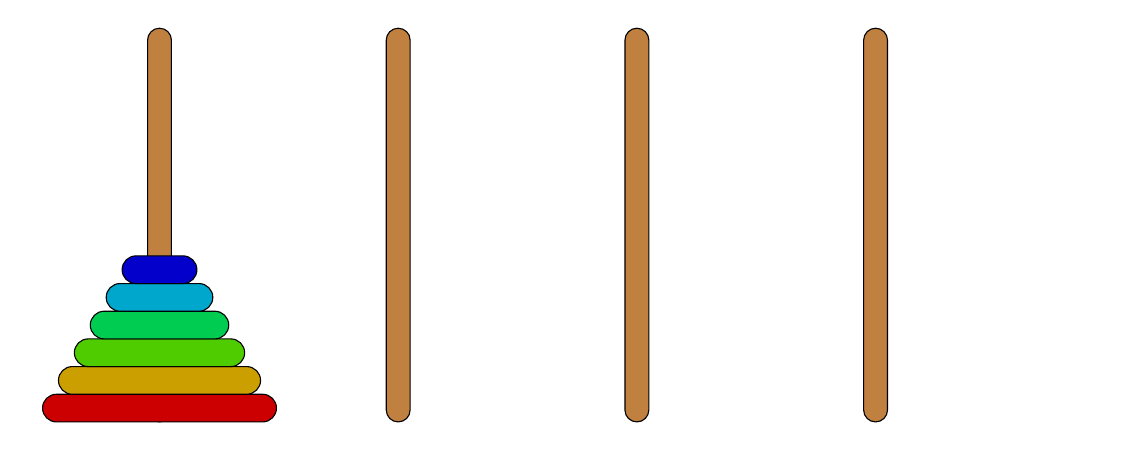
\begin{tikzpicture}
\pgfmathsetlengthmacro\diskheight{10};
\pgfmathsetmacro\k{4};
\pgfmathsetlengthmacro\step{\textwidth/\k};
\draw[color = white] (\step/2,0) -- (\textwidth+\step,0);
\foreach \n in {1,...,\k} \draw [fill = brown, draw = black, rounded corners = \step/20] (\step*\n,0) rectangle (\step*\n+\step/10,5);
\definecolor{mycolor}{rgb:hsb}{0.00,1,0.8}
\draw [fill = mycolor, draw = black, rounded corners = \diskheight/2] (\step*1+\step/20-\step*0.49,\diskheight*0) rectangle (\step*1+\step/20+\step*0.49,\diskheight*1);
\definecolor{mycolor}{rgb:hsb}{0.13,1,0.8}
\draw [fill = mycolor, draw = black, rounded corners = \diskheight/2] (\step*1+\step/20-\step*0.42333333333333334,\diskheight*1) rectangle (\step*1+\step/20+\step*0.42333333333333334,\diskheight*2);
\definecolor{mycolor}{rgb:hsb}{0.27,1,0.8}
\draw [fill = mycolor, draw = black, rounded corners = \diskheight/2] (\step*1+\step/20-\step*0.3566666666666667,\diskheight*2) rectangle (\step*1+\step/20+\step*0.3566666666666667,\diskheight*3);
\definecolor{mycolor}{rgb:hsb}{0.40,1,0.8}
\draw [fill = mycolor, draw = black, rounded corners = \diskheight/2] (\step*1+\step/20-\step*0.2899999999999999,\diskheight*3) rectangle (\step*1+\step/20+\step*0.2899999999999999,\diskheight*4);
\definecolor{mycolor}{rgb:hsb}{0.53,1,0.8}
\draw [fill = mycolor, draw = black, rounded corners = \diskheight/2] (\step*1+\step/20-\step*0.22333333333333333,\diskheight*4) rectangle (\step*1+\step/20+\step*0.22333333333333333,\diskheight*5);
\definecolor{mycolor}{rgb:hsb}{0.67,1,0.8}
\draw [fill = mycolor, draw = black, rounded corners = \diskheight/2] (\step*1+\step/20-\step*0.15666666666666668,\diskheight*5) rectangle (\step*1+\step/20+\step*0.15666666666666668,\diskheight*6);
\end{tikzpicture}
}
\only<2>{
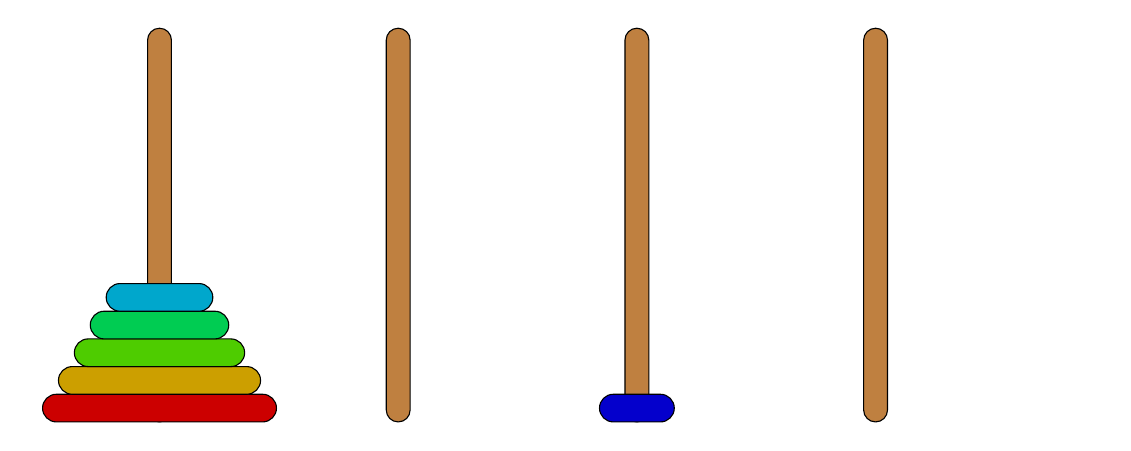
\begin{tikzpicture}
\pgfmathsetlengthmacro\diskheight{10};
\pgfmathsetmacro\k{4};
\pgfmathsetlengthmacro\step{\textwidth/\k};
\draw[color = white] (\step/2,0) -- (\textwidth+\step,0);
\foreach \n in {1,...,\k} \draw [fill = brown, draw = black, rounded corners = \step/20] (\step*\n,0) rectangle (\step*\n+\step/10,5);
\definecolor{mycolor}{rgb:hsb}{0.00,1,0.8}
\draw [fill = mycolor, draw = black, rounded corners = \diskheight/2] (\step*1+\step/20-\step*0.49,\diskheight*0) rectangle (\step*1+\step/20+\step*0.49,\diskheight*1);
\definecolor{mycolor}{rgb:hsb}{0.13,1,0.8}
\draw [fill = mycolor, draw = black, rounded corners = \diskheight/2] (\step*1+\step/20-\step*0.42333333333333334,\diskheight*1) rectangle (\step*1+\step/20+\step*0.42333333333333334,\diskheight*2);
\definecolor{mycolor}{rgb:hsb}{0.27,1,0.8}
\draw [fill = mycolor, draw = black, rounded corners = \diskheight/2] (\step*1+\step/20-\step*0.3566666666666667,\diskheight*2) rectangle (\step*1+\step/20+\step*0.3566666666666667,\diskheight*3);
\definecolor{mycolor}{rgb:hsb}{0.40,1,0.8}
\draw [fill = mycolor, draw = black, rounded corners = \diskheight/2] (\step*1+\step/20-\step*0.2899999999999999,\diskheight*3) rectangle (\step*1+\step/20+\step*0.2899999999999999,\diskheight*4);
\definecolor{mycolor}{rgb:hsb}{0.53,1,0.8}
\draw [fill = mycolor, draw = black, rounded corners = \diskheight/2] (\step*1+\step/20-\step*0.22333333333333333,\diskheight*4) rectangle (\step*1+\step/20+\step*0.22333333333333333,\diskheight*5);
\definecolor{mycolor}{rgb:hsb}{0.67,1,0.8}
\draw [fill = mycolor, draw = black, rounded corners = \diskheight/2] (\step*3+\step/20-\step*0.15666666666666668,\diskheight*0) rectangle (\step*3+\step/20+\step*0.15666666666666668,\diskheight*1);
\end{tikzpicture}
}
\only<3>{
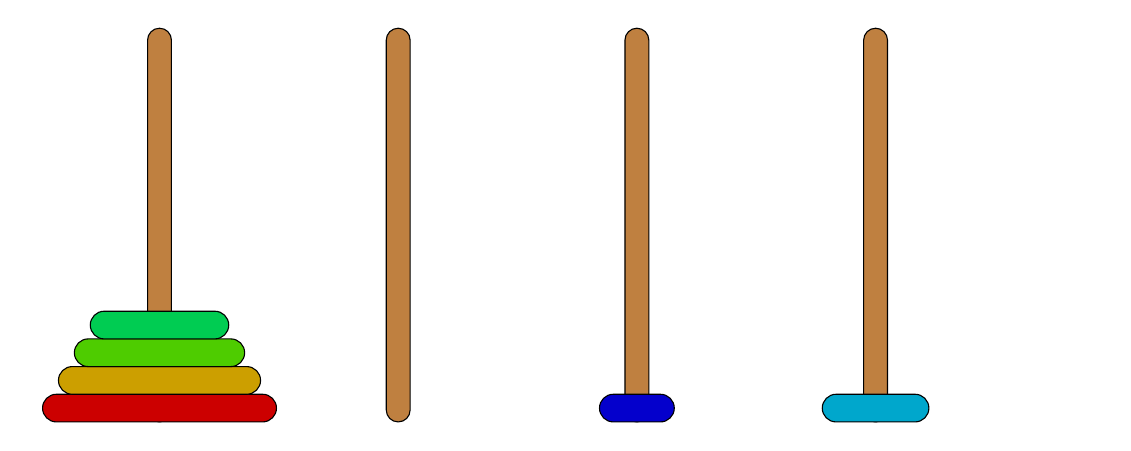
\begin{tikzpicture}
\pgfmathsetlengthmacro\diskheight{10};
\pgfmathsetmacro\k{4};
\pgfmathsetlengthmacro\step{\textwidth/\k};
\draw[color = white] (\step/2,0) -- (\textwidth+\step,0);
\foreach \n in {1,...,\k} \draw [fill = brown, draw = black, rounded corners = \step/20] (\step*\n,0) rectangle (\step*\n+\step/10,5);
\definecolor{mycolor}{rgb:hsb}{0.00,1,0.8}
\draw [fill = mycolor, draw = black, rounded corners = \diskheight/2] (\step*1+\step/20-\step*0.49,\diskheight*0) rectangle (\step*1+\step/20+\step*0.49,\diskheight*1);
\definecolor{mycolor}{rgb:hsb}{0.13,1,0.8}
\draw [fill = mycolor, draw = black, rounded corners = \diskheight/2] (\step*1+\step/20-\step*0.42333333333333334,\diskheight*1) rectangle (\step*1+\step/20+\step*0.42333333333333334,\diskheight*2);
\definecolor{mycolor}{rgb:hsb}{0.27,1,0.8}
\draw [fill = mycolor, draw = black, rounded corners = \diskheight/2] (\step*1+\step/20-\step*0.3566666666666667,\diskheight*2) rectangle (\step*1+\step/20+\step*0.3566666666666667,\diskheight*3);
\definecolor{mycolor}{rgb:hsb}{0.40,1,0.8}
\draw [fill = mycolor, draw = black, rounded corners = \diskheight/2] (\step*1+\step/20-\step*0.2899999999999999,\diskheight*3) rectangle (\step*1+\step/20+\step*0.2899999999999999,\diskheight*4);
\definecolor{mycolor}{rgb:hsb}{0.67,1,0.8}
\draw [fill = mycolor, draw = black, rounded corners = \diskheight/2] (\step*3+\step/20-\step*0.15666666666666668,\diskheight*0) rectangle (\step*3+\step/20+\step*0.15666666666666668,\diskheight*1);
\definecolor{mycolor}{rgb:hsb}{0.53,1,0.8}
\draw [fill = mycolor, draw = black, rounded corners = \diskheight/2] (\step*4+\step/20-\step*0.22333333333333333,\diskheight*0) rectangle (\step*4+\step/20+\step*0.22333333333333333,\diskheight*1);
\end{tikzpicture}
}
\only<4>{
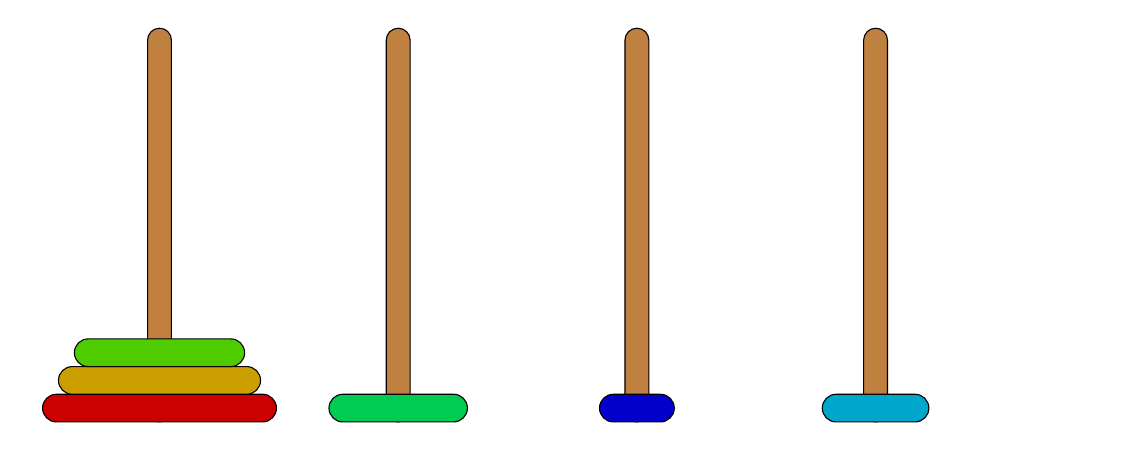
\begin{tikzpicture}
\pgfmathsetlengthmacro\diskheight{10};
\pgfmathsetmacro\k{4};
\pgfmathsetlengthmacro\step{\textwidth/\k};
\draw[color = white] (\step/2,0) -- (\textwidth+\step,0);
\foreach \n in {1,...,\k} \draw [fill = brown, draw = black, rounded corners = \step/20] (\step*\n,0) rectangle (\step*\n+\step/10,5);
\definecolor{mycolor}{rgb:hsb}{0.00,1,0.8}
\draw [fill = mycolor, draw = black, rounded corners = \diskheight/2] (\step*1+\step/20-\step*0.49,\diskheight*0) rectangle (\step*1+\step/20+\step*0.49,\diskheight*1);
\definecolor{mycolor}{rgb:hsb}{0.13,1,0.8}
\draw [fill = mycolor, draw = black, rounded corners = \diskheight/2] (\step*1+\step/20-\step*0.42333333333333334,\diskheight*1) rectangle (\step*1+\step/20+\step*0.42333333333333334,\diskheight*2);
\definecolor{mycolor}{rgb:hsb}{0.27,1,0.8}
\draw [fill = mycolor, draw = black, rounded corners = \diskheight/2] (\step*1+\step/20-\step*0.3566666666666667,\diskheight*2) rectangle (\step*1+\step/20+\step*0.3566666666666667,\diskheight*3);
\definecolor{mycolor}{rgb:hsb}{0.40,1,0.8}
\draw [fill = mycolor, draw = black, rounded corners = \diskheight/2] (\step*2+\step/20-\step*0.2899999999999999,\diskheight*0) rectangle (\step*2+\step/20+\step*0.2899999999999999,\diskheight*1);
\definecolor{mycolor}{rgb:hsb}{0.67,1,0.8}
\draw [fill = mycolor, draw = black, rounded corners = \diskheight/2] (\step*3+\step/20-\step*0.15666666666666668,\diskheight*0) rectangle (\step*3+\step/20+\step*0.15666666666666668,\diskheight*1);
\definecolor{mycolor}{rgb:hsb}{0.53,1,0.8}
\draw [fill = mycolor, draw = black, rounded corners = \diskheight/2] (\step*4+\step/20-\step*0.22333333333333333,\diskheight*0) rectangle (\step*4+\step/20+\step*0.22333333333333333,\diskheight*1);
\end{tikzpicture}
}
\only<5>{
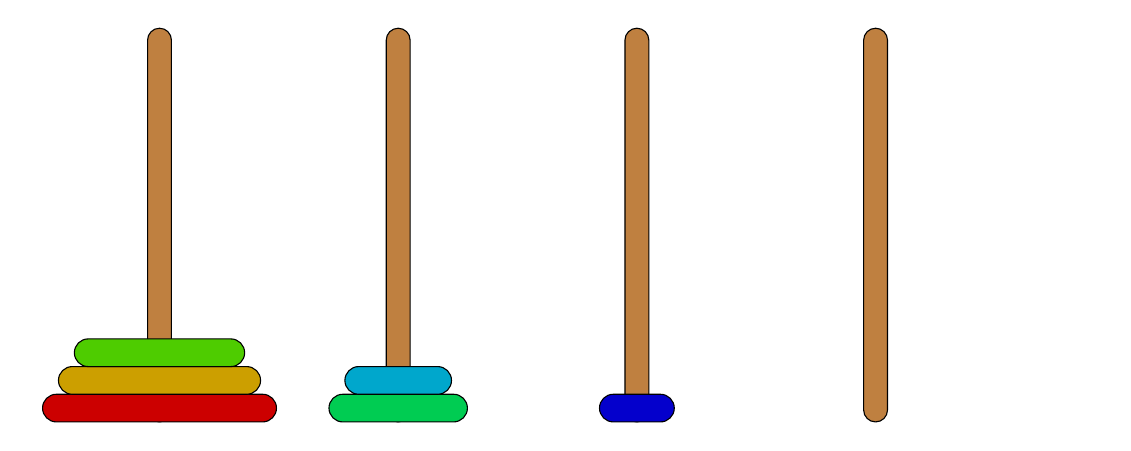
\begin{tikzpicture}
\pgfmathsetlengthmacro\diskheight{10};
\pgfmathsetmacro\k{4};
\pgfmathsetlengthmacro\step{\textwidth/\k};
\draw[color = white] (\step/2,0) -- (\textwidth+\step,0);
\foreach \n in {1,...,\k} \draw [fill = brown, draw = black, rounded corners = \step/20] (\step*\n,0) rectangle (\step*\n+\step/10,5);
\definecolor{mycolor}{rgb:hsb}{0.00,1,0.8}
\draw [fill = mycolor, draw = black, rounded corners = \diskheight/2] (\step*1+\step/20-\step*0.49,\diskheight*0) rectangle (\step*1+\step/20+\step*0.49,\diskheight*1);
\definecolor{mycolor}{rgb:hsb}{0.13,1,0.8}
\draw [fill = mycolor, draw = black, rounded corners = \diskheight/2] (\step*1+\step/20-\step*0.42333333333333334,\diskheight*1) rectangle (\step*1+\step/20+\step*0.42333333333333334,\diskheight*2);
\definecolor{mycolor}{rgb:hsb}{0.27,1,0.8}
\draw [fill = mycolor, draw = black, rounded corners = \diskheight/2] (\step*1+\step/20-\step*0.3566666666666667,\diskheight*2) rectangle (\step*1+\step/20+\step*0.3566666666666667,\diskheight*3);
\definecolor{mycolor}{rgb:hsb}{0.40,1,0.8}
\draw [fill = mycolor, draw = black, rounded corners = \diskheight/2] (\step*2+\step/20-\step*0.2899999999999999,\diskheight*0) rectangle (\step*2+\step/20+\step*0.2899999999999999,\diskheight*1);
\definecolor{mycolor}{rgb:hsb}{0.53,1,0.8}
\draw [fill = mycolor, draw = black, rounded corners = \diskheight/2] (\step*2+\step/20-\step*0.22333333333333333,\diskheight*1) rectangle (\step*2+\step/20+\step*0.22333333333333333,\diskheight*2);
\definecolor{mycolor}{rgb:hsb}{0.67,1,0.8}
\draw [fill = mycolor, draw = black, rounded corners = \diskheight/2] (\step*3+\step/20-\step*0.15666666666666668,\diskheight*0) rectangle (\step*3+\step/20+\step*0.15666666666666668,\diskheight*1);
\end{tikzpicture}
}
\only<6>{
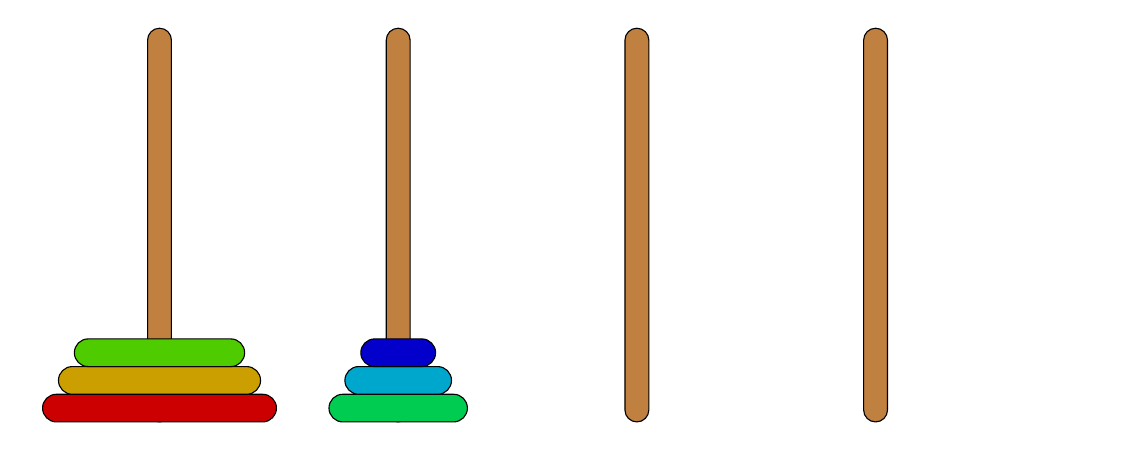
\begin{tikzpicture}
\pgfmathsetlengthmacro\diskheight{10};
\pgfmathsetmacro\k{4};
\pgfmathsetlengthmacro\step{\textwidth/\k};
\draw[color = white] (\step/2,0) -- (\textwidth+\step,0);
\foreach \n in {1,...,\k} \draw [fill = brown, draw = black, rounded corners = \step/20] (\step*\n,0) rectangle (\step*\n+\step/10,5);
\definecolor{mycolor}{rgb:hsb}{0.00,1,0.8}
\draw [fill = mycolor, draw = black, rounded corners = \diskheight/2] (\step*1+\step/20-\step*0.49,\diskheight*0) rectangle (\step*1+\step/20+\step*0.49,\diskheight*1);
\definecolor{mycolor}{rgb:hsb}{0.13,1,0.8}
\draw [fill = mycolor, draw = black, rounded corners = \diskheight/2] (\step*1+\step/20-\step*0.42333333333333334,\diskheight*1) rectangle (\step*1+\step/20+\step*0.42333333333333334,\diskheight*2);
\definecolor{mycolor}{rgb:hsb}{0.27,1,0.8}
\draw [fill = mycolor, draw = black, rounded corners = \diskheight/2] (\step*1+\step/20-\step*0.3566666666666667,\diskheight*2) rectangle (\step*1+\step/20+\step*0.3566666666666667,\diskheight*3);
\definecolor{mycolor}{rgb:hsb}{0.40,1,0.8}
\draw [fill = mycolor, draw = black, rounded corners = \diskheight/2] (\step*2+\step/20-\step*0.2899999999999999,\diskheight*0) rectangle (\step*2+\step/20+\step*0.2899999999999999,\diskheight*1);
\definecolor{mycolor}{rgb:hsb}{0.53,1,0.8}
\draw [fill = mycolor, draw = black, rounded corners = \diskheight/2] (\step*2+\step/20-\step*0.22333333333333333,\diskheight*1) rectangle (\step*2+\step/20+\step*0.22333333333333333,\diskheight*2);
\definecolor{mycolor}{rgb:hsb}{0.67,1,0.8}
\draw [fill = mycolor, draw = black, rounded corners = \diskheight/2] (\step*2+\step/20-\step*0.15666666666666668,\diskheight*2) rectangle (\step*2+\step/20+\step*0.15666666666666668,\diskheight*3);
\end{tikzpicture}
}
\only<7>{
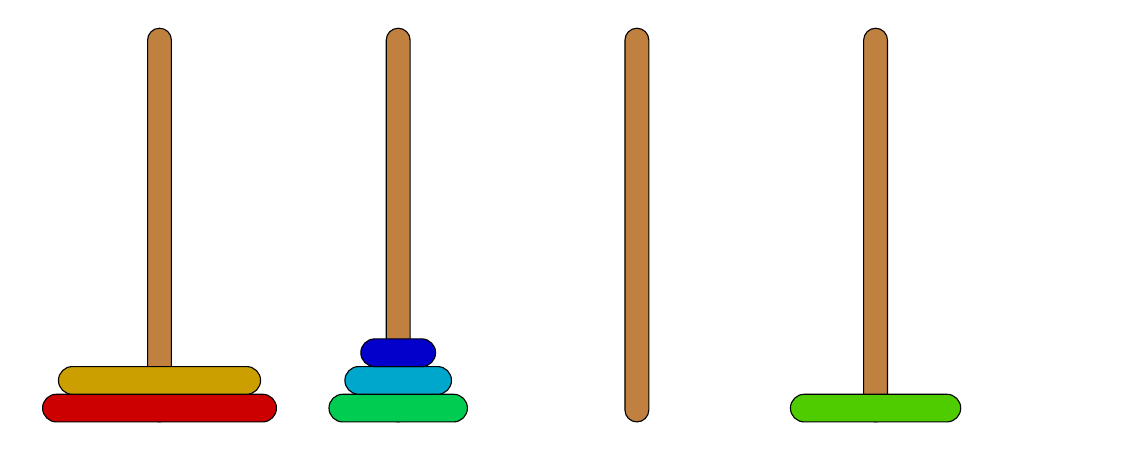
\begin{tikzpicture}
\pgfmathsetlengthmacro\diskheight{10};
\pgfmathsetmacro\k{4};
\pgfmathsetlengthmacro\step{\textwidth/\k};
\draw[color = white] (\step/2,0) -- (\textwidth+\step,0);
\foreach \n in {1,...,\k} \draw [fill = brown, draw = black, rounded corners = \step/20] (\step*\n,0) rectangle (\step*\n+\step/10,5);
\definecolor{mycolor}{rgb:hsb}{0.00,1,0.8}
\draw [fill = mycolor, draw = black, rounded corners = \diskheight/2] (\step*1+\step/20-\step*0.49,\diskheight*0) rectangle (\step*1+\step/20+\step*0.49,\diskheight*1);
\definecolor{mycolor}{rgb:hsb}{0.13,1,0.8}
\draw [fill = mycolor, draw = black, rounded corners = \diskheight/2] (\step*1+\step/20-\step*0.42333333333333334,\diskheight*1) rectangle (\step*1+\step/20+\step*0.42333333333333334,\diskheight*2);
\definecolor{mycolor}{rgb:hsb}{0.40,1,0.8}
\draw [fill = mycolor, draw = black, rounded corners = \diskheight/2] (\step*2+\step/20-\step*0.2899999999999999,\diskheight*0) rectangle (\step*2+\step/20+\step*0.2899999999999999,\diskheight*1);
\definecolor{mycolor}{rgb:hsb}{0.53,1,0.8}
\draw [fill = mycolor, draw = black, rounded corners = \diskheight/2] (\step*2+\step/20-\step*0.22333333333333333,\diskheight*1) rectangle (\step*2+\step/20+\step*0.22333333333333333,\diskheight*2);
\definecolor{mycolor}{rgb:hsb}{0.67,1,0.8}
\draw [fill = mycolor, draw = black, rounded corners = \diskheight/2] (\step*2+\step/20-\step*0.15666666666666668,\diskheight*2) rectangle (\step*2+\step/20+\step*0.15666666666666668,\diskheight*3);
\definecolor{mycolor}{rgb:hsb}{0.27,1,0.8}
\draw [fill = mycolor, draw = black, rounded corners = \diskheight/2] (\step*4+\step/20-\step*0.3566666666666667,\diskheight*0) rectangle (\step*4+\step/20+\step*0.3566666666666667,\diskheight*1);
\end{tikzpicture}
}
\only<8>{
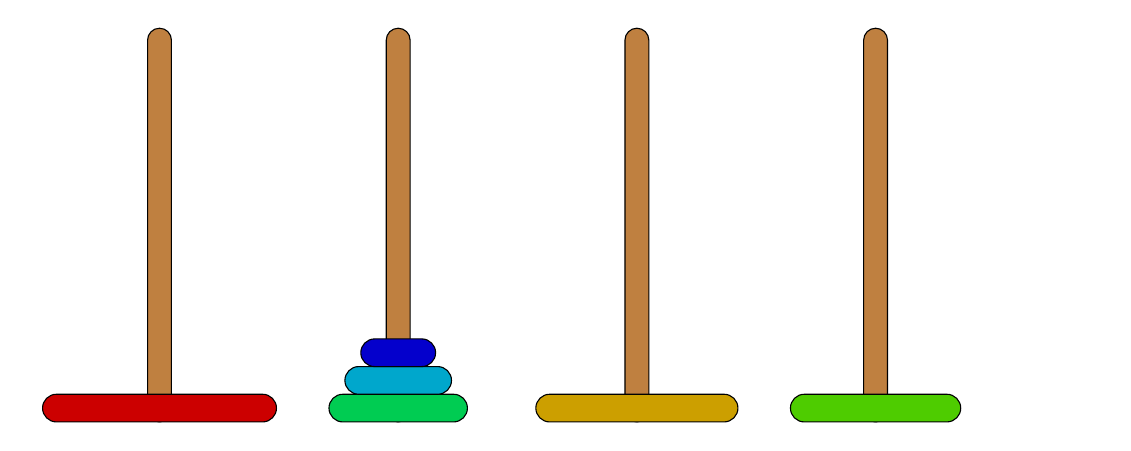
\begin{tikzpicture}
\pgfmathsetlengthmacro\diskheight{10};
\pgfmathsetmacro\k{4};
\pgfmathsetlengthmacro\step{\textwidth/\k};
\draw[color = white] (\step/2,0) -- (\textwidth+\step,0);
\foreach \n in {1,...,\k} \draw [fill = brown, draw = black, rounded corners = \step/20] (\step*\n,0) rectangle (\step*\n+\step/10,5);
\definecolor{mycolor}{rgb:hsb}{0.00,1,0.8}
\draw [fill = mycolor, draw = black, rounded corners = \diskheight/2] (\step*1+\step/20-\step*0.49,\diskheight*0) rectangle (\step*1+\step/20+\step*0.49,\diskheight*1);
\definecolor{mycolor}{rgb:hsb}{0.40,1,0.8}
\draw [fill = mycolor, draw = black, rounded corners = \diskheight/2] (\step*2+\step/20-\step*0.2899999999999999,\diskheight*0) rectangle (\step*2+\step/20+\step*0.2899999999999999,\diskheight*1);
\definecolor{mycolor}{rgb:hsb}{0.53,1,0.8}
\draw [fill = mycolor, draw = black, rounded corners = \diskheight/2] (\step*2+\step/20-\step*0.22333333333333333,\diskheight*1) rectangle (\step*2+\step/20+\step*0.22333333333333333,\diskheight*2);
\definecolor{mycolor}{rgb:hsb}{0.67,1,0.8}
\draw [fill = mycolor, draw = black, rounded corners = \diskheight/2] (\step*2+\step/20-\step*0.15666666666666668,\diskheight*2) rectangle (\step*2+\step/20+\step*0.15666666666666668,\diskheight*3);
\definecolor{mycolor}{rgb:hsb}{0.13,1,0.8}
\draw [fill = mycolor, draw = black, rounded corners = \diskheight/2] (\step*3+\step/20-\step*0.42333333333333334,\diskheight*0) rectangle (\step*3+\step/20+\step*0.42333333333333334,\diskheight*1);
\definecolor{mycolor}{rgb:hsb}{0.27,1,0.8}
\draw [fill = mycolor, draw = black, rounded corners = \diskheight/2] (\step*4+\step/20-\step*0.3566666666666667,\diskheight*0) rectangle (\step*4+\step/20+\step*0.3566666666666667,\diskheight*1);
\end{tikzpicture}
}
\only<9>{
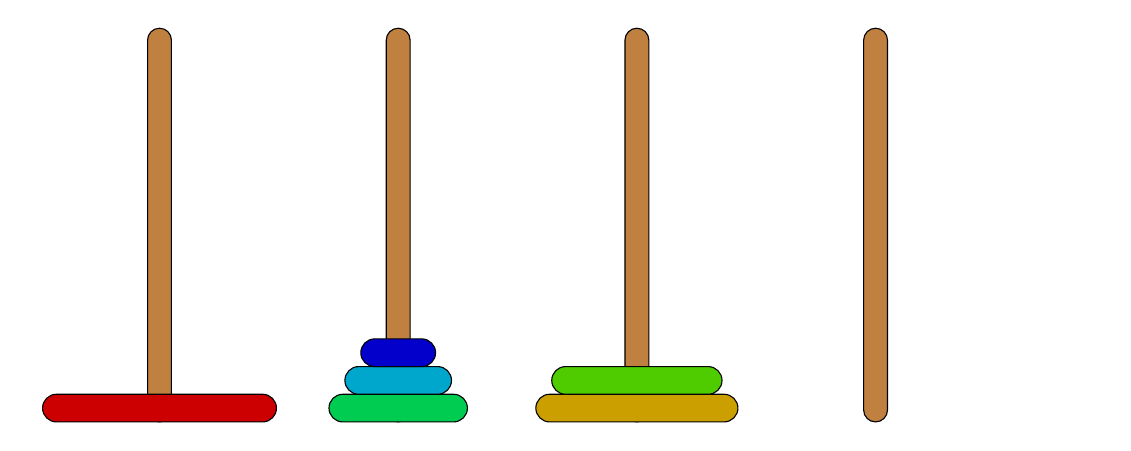
\begin{tikzpicture}
\pgfmathsetlengthmacro\diskheight{10};
\pgfmathsetmacro\k{4};
\pgfmathsetlengthmacro\step{\textwidth/\k};
\draw[color = white] (\step/2,0) -- (\textwidth+\step,0);
\foreach \n in {1,...,\k} \draw [fill = brown, draw = black, rounded corners = \step/20] (\step*\n,0) rectangle (\step*\n+\step/10,5);
\definecolor{mycolor}{rgb:hsb}{0.00,1,0.8}
\draw [fill = mycolor, draw = black, rounded corners = \diskheight/2] (\step*1+\step/20-\step*0.49,\diskheight*0) rectangle (\step*1+\step/20+\step*0.49,\diskheight*1);
\definecolor{mycolor}{rgb:hsb}{0.40,1,0.8}
\draw [fill = mycolor, draw = black, rounded corners = \diskheight/2] (\step*2+\step/20-\step*0.2899999999999999,\diskheight*0) rectangle (\step*2+\step/20+\step*0.2899999999999999,\diskheight*1);
\definecolor{mycolor}{rgb:hsb}{0.53,1,0.8}
\draw [fill = mycolor, draw = black, rounded corners = \diskheight/2] (\step*2+\step/20-\step*0.22333333333333333,\diskheight*1) rectangle (\step*2+\step/20+\step*0.22333333333333333,\diskheight*2);
\definecolor{mycolor}{rgb:hsb}{0.67,1,0.8}
\draw [fill = mycolor, draw = black, rounded corners = \diskheight/2] (\step*2+\step/20-\step*0.15666666666666668,\diskheight*2) rectangle (\step*2+\step/20+\step*0.15666666666666668,\diskheight*3);
\definecolor{mycolor}{rgb:hsb}{0.13,1,0.8}
\draw [fill = mycolor, draw = black, rounded corners = \diskheight/2] (\step*3+\step/20-\step*0.42333333333333334,\diskheight*0) rectangle (\step*3+\step/20+\step*0.42333333333333334,\diskheight*1);
\definecolor{mycolor}{rgb:hsb}{0.27,1,0.8}
\draw [fill = mycolor, draw = black, rounded corners = \diskheight/2] (\step*3+\step/20-\step*0.3566666666666667,\diskheight*1) rectangle (\step*3+\step/20+\step*0.3566666666666667,\diskheight*2);
\end{tikzpicture}
}
\only<10>{
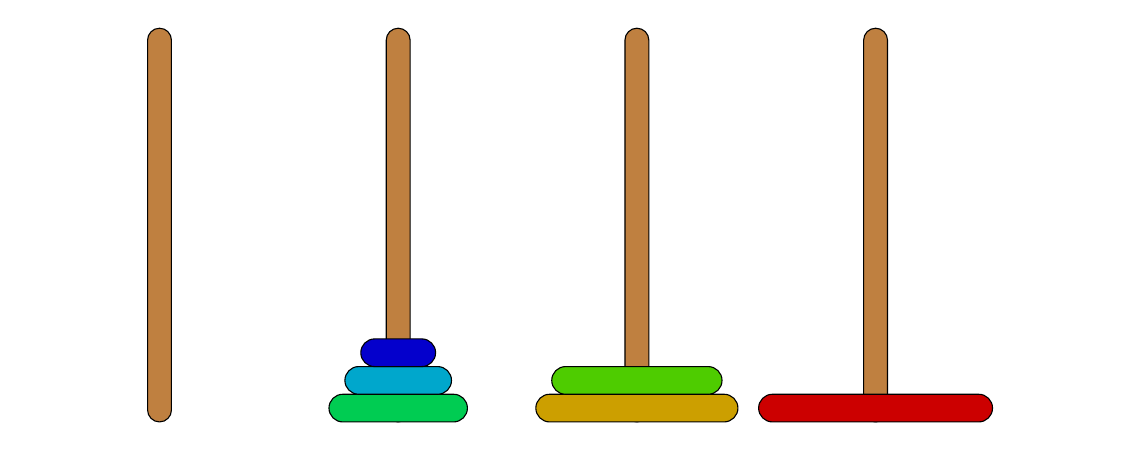
\begin{tikzpicture}
\pgfmathsetlengthmacro\diskheight{10};
\pgfmathsetmacro\k{4};
\pgfmathsetlengthmacro\step{\textwidth/\k};
\draw[color = white] (\step/2,0) -- (\textwidth+\step,0);
\foreach \n in {1,...,\k} \draw [fill = brown, draw = black, rounded corners = \step/20] (\step*\n,0) rectangle (\step*\n+\step/10,5);
\definecolor{mycolor}{rgb:hsb}{0.40,1,0.8}
\draw [fill = mycolor, draw = black, rounded corners = \diskheight/2] (\step*2+\step/20-\step*0.2899999999999999,\diskheight*0) rectangle (\step*2+\step/20+\step*0.2899999999999999,\diskheight*1);
\definecolor{mycolor}{rgb:hsb}{0.53,1,0.8}
\draw [fill = mycolor, draw = black, rounded corners = \diskheight/2] (\step*2+\step/20-\step*0.22333333333333333,\diskheight*1) rectangle (\step*2+\step/20+\step*0.22333333333333333,\diskheight*2);
\definecolor{mycolor}{rgb:hsb}{0.67,1,0.8}
\draw [fill = mycolor, draw = black, rounded corners = \diskheight/2] (\step*2+\step/20-\step*0.15666666666666668,\diskheight*2) rectangle (\step*2+\step/20+\step*0.15666666666666668,\diskheight*3);
\definecolor{mycolor}{rgb:hsb}{0.13,1,0.8}
\draw [fill = mycolor, draw = black, rounded corners = \diskheight/2] (\step*3+\step/20-\step*0.42333333333333334,\diskheight*0) rectangle (\step*3+\step/20+\step*0.42333333333333334,\diskheight*1);
\definecolor{mycolor}{rgb:hsb}{0.27,1,0.8}
\draw [fill = mycolor, draw = black, rounded corners = \diskheight/2] (\step*3+\step/20-\step*0.3566666666666667,\diskheight*1) rectangle (\step*3+\step/20+\step*0.3566666666666667,\diskheight*2);
\definecolor{mycolor}{rgb:hsb}{0.00,1,0.8}
\draw [fill = mycolor, draw = black, rounded corners = \diskheight/2] (\step*4+\step/20-\step*0.49,\diskheight*0) rectangle (\step*4+\step/20+\step*0.49,\diskheight*1);
\end{tikzpicture}
}
\only<11>{
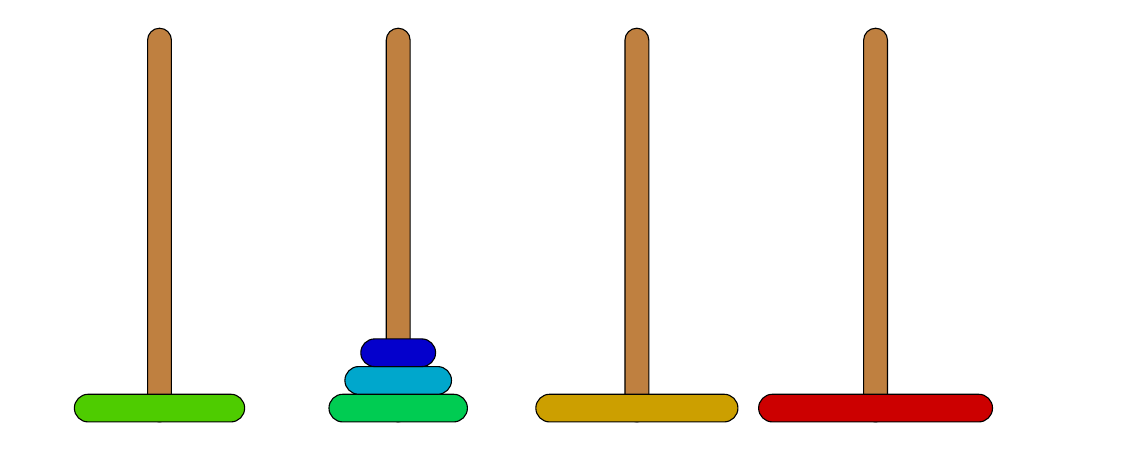
\begin{tikzpicture}
\pgfmathsetlengthmacro\diskheight{10};
\pgfmathsetmacro\k{4};
\pgfmathsetlengthmacro\step{\textwidth/\k};
\draw[color = white] (\step/2,0) -- (\textwidth+\step,0);
\foreach \n in {1,...,\k} \draw [fill = brown, draw = black, rounded corners = \step/20] (\step*\n,0) rectangle (\step*\n+\step/10,5);
\definecolor{mycolor}{rgb:hsb}{0.27,1,0.8}
\draw [fill = mycolor, draw = black, rounded corners = \diskheight/2] (\step*1+\step/20-\step*0.3566666666666667,\diskheight*0) rectangle (\step*1+\step/20+\step*0.3566666666666667,\diskheight*1);
\definecolor{mycolor}{rgb:hsb}{0.40,1,0.8}
\draw [fill = mycolor, draw = black, rounded corners = \diskheight/2] (\step*2+\step/20-\step*0.2899999999999999,\diskheight*0) rectangle (\step*2+\step/20+\step*0.2899999999999999,\diskheight*1);
\definecolor{mycolor}{rgb:hsb}{0.53,1,0.8}
\draw [fill = mycolor, draw = black, rounded corners = \diskheight/2] (\step*2+\step/20-\step*0.22333333333333333,\diskheight*1) rectangle (\step*2+\step/20+\step*0.22333333333333333,\diskheight*2);
\definecolor{mycolor}{rgb:hsb}{0.67,1,0.8}
\draw [fill = mycolor, draw = black, rounded corners = \diskheight/2] (\step*2+\step/20-\step*0.15666666666666668,\diskheight*2) rectangle (\step*2+\step/20+\step*0.15666666666666668,\diskheight*3);
\definecolor{mycolor}{rgb:hsb}{0.13,1,0.8}
\draw [fill = mycolor, draw = black, rounded corners = \diskheight/2] (\step*3+\step/20-\step*0.42333333333333334,\diskheight*0) rectangle (\step*3+\step/20+\step*0.42333333333333334,\diskheight*1);
\definecolor{mycolor}{rgb:hsb}{0.00,1,0.8}
\draw [fill = mycolor, draw = black, rounded corners = \diskheight/2] (\step*4+\step/20-\step*0.49,\diskheight*0) rectangle (\step*4+\step/20+\step*0.49,\diskheight*1);
\end{tikzpicture}
}
\only<12>{
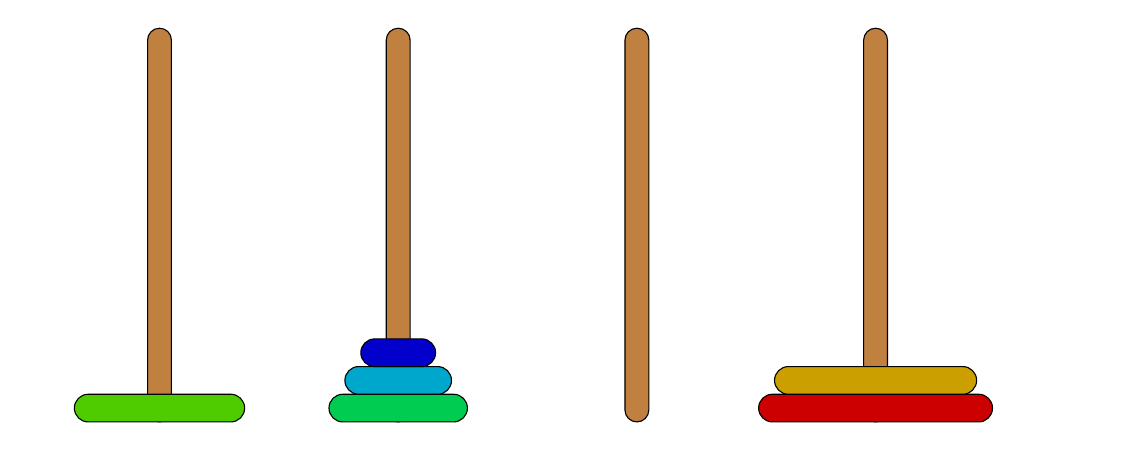
\begin{tikzpicture}
\pgfmathsetlengthmacro\diskheight{10};
\pgfmathsetmacro\k{4};
\pgfmathsetlengthmacro\step{\textwidth/\k};
\draw[color = white] (\step/2,0) -- (\textwidth+\step,0);
\foreach \n in {1,...,\k} \draw [fill = brown, draw = black, rounded corners = \step/20] (\step*\n,0) rectangle (\step*\n+\step/10,5);
\definecolor{mycolor}{rgb:hsb}{0.27,1,0.8}
\draw [fill = mycolor, draw = black, rounded corners = \diskheight/2] (\step*1+\step/20-\step*0.3566666666666667,\diskheight*0) rectangle (\step*1+\step/20+\step*0.3566666666666667,\diskheight*1);
\definecolor{mycolor}{rgb:hsb}{0.40,1,0.8}
\draw [fill = mycolor, draw = black, rounded corners = \diskheight/2] (\step*2+\step/20-\step*0.2899999999999999,\diskheight*0) rectangle (\step*2+\step/20+\step*0.2899999999999999,\diskheight*1);
\definecolor{mycolor}{rgb:hsb}{0.53,1,0.8}
\draw [fill = mycolor, draw = black, rounded corners = \diskheight/2] (\step*2+\step/20-\step*0.22333333333333333,\diskheight*1) rectangle (\step*2+\step/20+\step*0.22333333333333333,\diskheight*2);
\definecolor{mycolor}{rgb:hsb}{0.67,1,0.8}
\draw [fill = mycolor, draw = black, rounded corners = \diskheight/2] (\step*2+\step/20-\step*0.15666666666666668,\diskheight*2) rectangle (\step*2+\step/20+\step*0.15666666666666668,\diskheight*3);
\definecolor{mycolor}{rgb:hsb}{0.00,1,0.8}
\draw [fill = mycolor, draw = black, rounded corners = \diskheight/2] (\step*4+\step/20-\step*0.49,\diskheight*0) rectangle (\step*4+\step/20+\step*0.49,\diskheight*1);
\definecolor{mycolor}{rgb:hsb}{0.13,1,0.8}
\draw [fill = mycolor, draw = black, rounded corners = \diskheight/2] (\step*4+\step/20-\step*0.42333333333333334,\diskheight*1) rectangle (\step*4+\step/20+\step*0.42333333333333334,\diskheight*2);
\end{tikzpicture}
}
\only<13>{
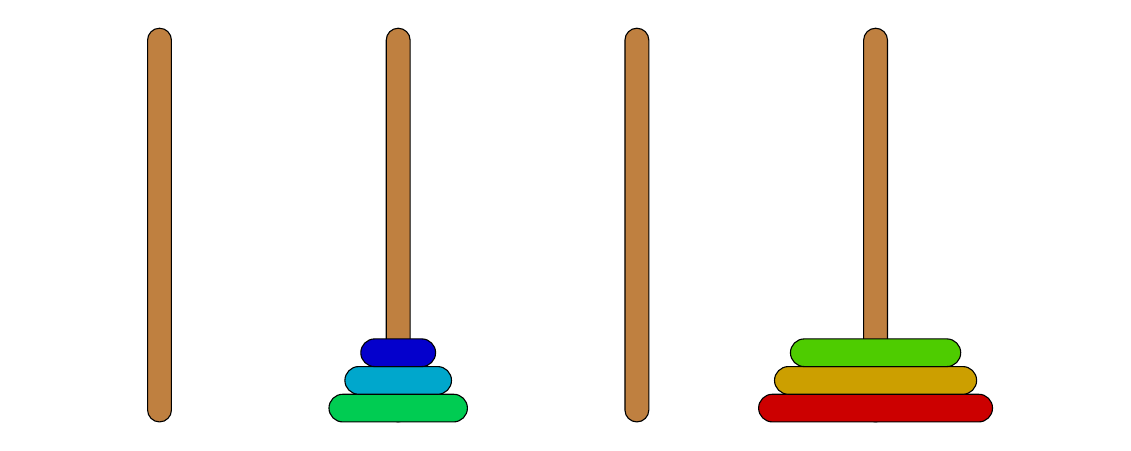
\begin{tikzpicture}
\pgfmathsetlengthmacro\diskheight{10};
\pgfmathsetmacro\k{4};
\pgfmathsetlengthmacro\step{\textwidth/\k};
\draw[color = white] (\step/2,0) -- (\textwidth+\step,0);
\foreach \n in {1,...,\k} \draw [fill = brown, draw = black, rounded corners = \step/20] (\step*\n,0) rectangle (\step*\n+\step/10,5);
\definecolor{mycolor}{rgb:hsb}{0.40,1,0.8}
\draw [fill = mycolor, draw = black, rounded corners = \diskheight/2] (\step*2+\step/20-\step*0.2899999999999999,\diskheight*0) rectangle (\step*2+\step/20+\step*0.2899999999999999,\diskheight*1);
\definecolor{mycolor}{rgb:hsb}{0.53,1,0.8}
\draw [fill = mycolor, draw = black, rounded corners = \diskheight/2] (\step*2+\step/20-\step*0.22333333333333333,\diskheight*1) rectangle (\step*2+\step/20+\step*0.22333333333333333,\diskheight*2);
\definecolor{mycolor}{rgb:hsb}{0.67,1,0.8}
\draw [fill = mycolor, draw = black, rounded corners = \diskheight/2] (\step*2+\step/20-\step*0.15666666666666668,\diskheight*2) rectangle (\step*2+\step/20+\step*0.15666666666666668,\diskheight*3);
\definecolor{mycolor}{rgb:hsb}{0.00,1,0.8}
\draw [fill = mycolor, draw = black, rounded corners = \diskheight/2] (\step*4+\step/20-\step*0.49,\diskheight*0) rectangle (\step*4+\step/20+\step*0.49,\diskheight*1);
\definecolor{mycolor}{rgb:hsb}{0.13,1,0.8}
\draw [fill = mycolor, draw = black, rounded corners = \diskheight/2] (\step*4+\step/20-\step*0.42333333333333334,\diskheight*1) rectangle (\step*4+\step/20+\step*0.42333333333333334,\diskheight*2);
\definecolor{mycolor}{rgb:hsb}{0.27,1,0.8}
\draw [fill = mycolor, draw = black, rounded corners = \diskheight/2] (\step*4+\step/20-\step*0.3566666666666667,\diskheight*2) rectangle (\step*4+\step/20+\step*0.3566666666666667,\diskheight*3);
\end{tikzpicture}
}
\only<14>{
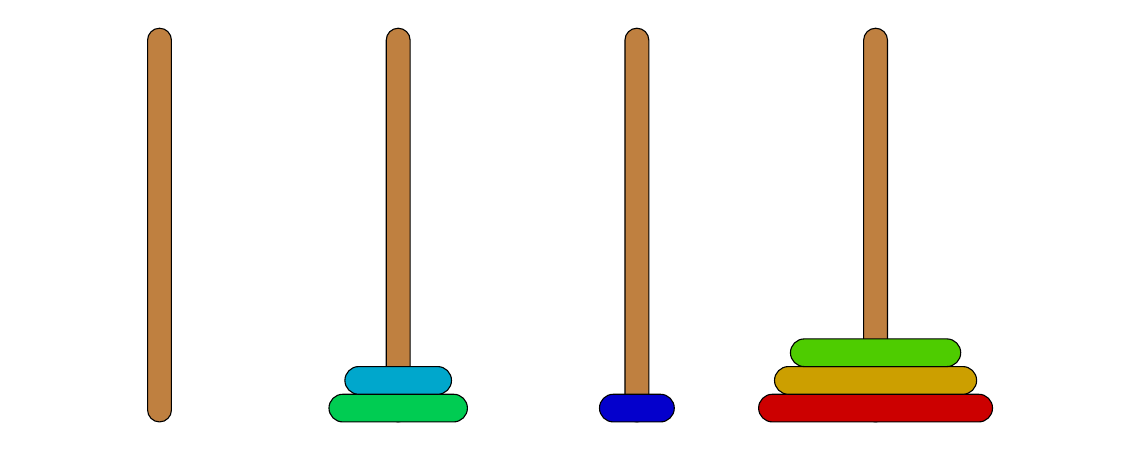
\begin{tikzpicture}
\pgfmathsetlengthmacro\diskheight{10};
\pgfmathsetmacro\k{4};
\pgfmathsetlengthmacro\step{\textwidth/\k};
\draw[color = white] (\step/2,0) -- (\textwidth+\step,0);
\foreach \n in {1,...,\k} \draw [fill = brown, draw = black, rounded corners = \step/20] (\step*\n,0) rectangle (\step*\n+\step/10,5);
\definecolor{mycolor}{rgb:hsb}{0.40,1,0.8}
\draw [fill = mycolor, draw = black, rounded corners = \diskheight/2] (\step*2+\step/20-\step*0.2899999999999999,\diskheight*0) rectangle (\step*2+\step/20+\step*0.2899999999999999,\diskheight*1);
\definecolor{mycolor}{rgb:hsb}{0.53,1,0.8}
\draw [fill = mycolor, draw = black, rounded corners = \diskheight/2] (\step*2+\step/20-\step*0.22333333333333333,\diskheight*1) rectangle (\step*2+\step/20+\step*0.22333333333333333,\diskheight*2);
\definecolor{mycolor}{rgb:hsb}{0.67,1,0.8}
\draw [fill = mycolor, draw = black, rounded corners = \diskheight/2] (\step*3+\step/20-\step*0.15666666666666668,\diskheight*0) rectangle (\step*3+\step/20+\step*0.15666666666666668,\diskheight*1);
\definecolor{mycolor}{rgb:hsb}{0.00,1,0.8}
\draw [fill = mycolor, draw = black, rounded corners = \diskheight/2] (\step*4+\step/20-\step*0.49,\diskheight*0) rectangle (\step*4+\step/20+\step*0.49,\diskheight*1);
\definecolor{mycolor}{rgb:hsb}{0.13,1,0.8}
\draw [fill = mycolor, draw = black, rounded corners = \diskheight/2] (\step*4+\step/20-\step*0.42333333333333334,\diskheight*1) rectangle (\step*4+\step/20+\step*0.42333333333333334,\diskheight*2);
\definecolor{mycolor}{rgb:hsb}{0.27,1,0.8}
\draw [fill = mycolor, draw = black, rounded corners = \diskheight/2] (\step*4+\step/20-\step*0.3566666666666667,\diskheight*2) rectangle (\step*4+\step/20+\step*0.3566666666666667,\diskheight*3);
\end{tikzpicture}
}
\only<15>{
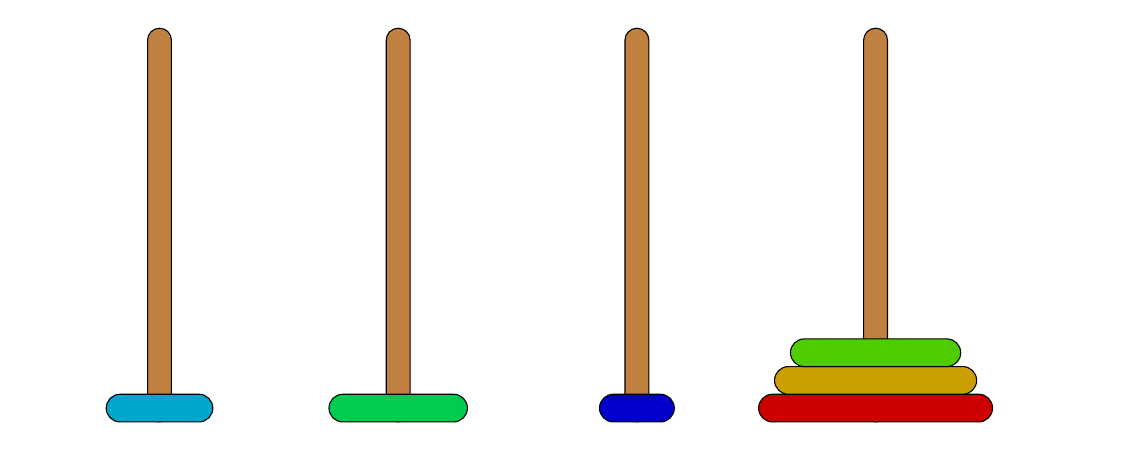
\begin{tikzpicture}
\pgfmathsetlengthmacro\diskheight{10};
\pgfmathsetmacro\k{4};
\pgfmathsetlengthmacro\step{\textwidth/\k};
\draw[color = white] (\step/2,0) -- (\textwidth+\step,0);
\foreach \n in {1,...,\k} \draw [fill = brown, draw = black, rounded corners = \step/20] (\step*\n,0) rectangle (\step*\n+\step/10,5);
\definecolor{mycolor}{rgb:hsb}{0.53,1,0.8}
\draw [fill = mycolor, draw = black, rounded corners = \diskheight/2] (\step*1+\step/20-\step*0.22333333333333333,\diskheight*0) rectangle (\step*1+\step/20+\step*0.22333333333333333,\diskheight*1);
\definecolor{mycolor}{rgb:hsb}{0.40,1,0.8}
\draw [fill = mycolor, draw = black, rounded corners = \diskheight/2] (\step*2+\step/20-\step*0.2899999999999999,\diskheight*0) rectangle (\step*2+\step/20+\step*0.2899999999999999,\diskheight*1);
\definecolor{mycolor}{rgb:hsb}{0.67,1,0.8}
\draw [fill = mycolor, draw = black, rounded corners = \diskheight/2] (\step*3+\step/20-\step*0.15666666666666668,\diskheight*0) rectangle (\step*3+\step/20+\step*0.15666666666666668,\diskheight*1);
\definecolor{mycolor}{rgb:hsb}{0.00,1,0.8}
\draw [fill = mycolor, draw = black, rounded corners = \diskheight/2] (\step*4+\step/20-\step*0.49,\diskheight*0) rectangle (\step*4+\step/20+\step*0.49,\diskheight*1);
\definecolor{mycolor}{rgb:hsb}{0.13,1,0.8}
\draw [fill = mycolor, draw = black, rounded corners = \diskheight/2] (\step*4+\step/20-\step*0.42333333333333334,\diskheight*1) rectangle (\step*4+\step/20+\step*0.42333333333333334,\diskheight*2);
\definecolor{mycolor}{rgb:hsb}{0.27,1,0.8}
\draw [fill = mycolor, draw = black, rounded corners = \diskheight/2] (\step*4+\step/20-\step*0.3566666666666667,\diskheight*2) rectangle (\step*4+\step/20+\step*0.3566666666666667,\diskheight*3);
\end{tikzpicture}
}
\only<16>{
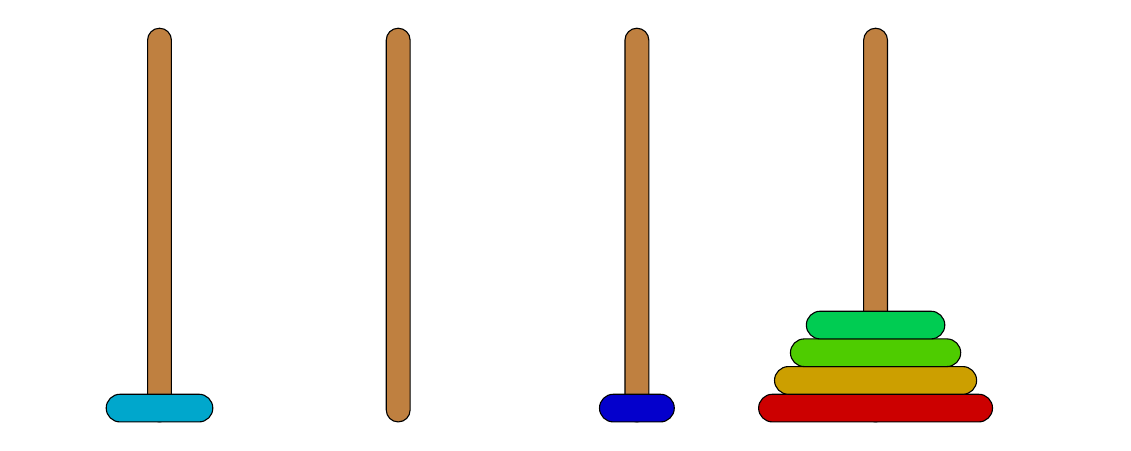
\begin{tikzpicture}
\pgfmathsetlengthmacro\diskheight{10};
\pgfmathsetmacro\k{4};
\pgfmathsetlengthmacro\step{\textwidth/\k};
\draw[color = white] (\step/2,0) -- (\textwidth+\step,0);
\foreach \n in {1,...,\k} \draw [fill = brown, draw = black, rounded corners = \step/20] (\step*\n,0) rectangle (\step*\n+\step/10,5);
\definecolor{mycolor}{rgb:hsb}{0.53,1,0.8}
\draw [fill = mycolor, draw = black, rounded corners = \diskheight/2] (\step*1+\step/20-\step*0.22333333333333333,\diskheight*0) rectangle (\step*1+\step/20+\step*0.22333333333333333,\diskheight*1);
\definecolor{mycolor}{rgb:hsb}{0.67,1,0.8}
\draw [fill = mycolor, draw = black, rounded corners = \diskheight/2] (\step*3+\step/20-\step*0.15666666666666668,\diskheight*0) rectangle (\step*3+\step/20+\step*0.15666666666666668,\diskheight*1);
\definecolor{mycolor}{rgb:hsb}{0.00,1,0.8}
\draw [fill = mycolor, draw = black, rounded corners = \diskheight/2] (\step*4+\step/20-\step*0.49,\diskheight*0) rectangle (\step*4+\step/20+\step*0.49,\diskheight*1);
\definecolor{mycolor}{rgb:hsb}{0.13,1,0.8}
\draw [fill = mycolor, draw = black, rounded corners = \diskheight/2] (\step*4+\step/20-\step*0.42333333333333334,\diskheight*1) rectangle (\step*4+\step/20+\step*0.42333333333333334,\diskheight*2);
\definecolor{mycolor}{rgb:hsb}{0.27,1,0.8}
\draw [fill = mycolor, draw = black, rounded corners = \diskheight/2] (\step*4+\step/20-\step*0.3566666666666667,\diskheight*2) rectangle (\step*4+\step/20+\step*0.3566666666666667,\diskheight*3);
\definecolor{mycolor}{rgb:hsb}{0.40,1,0.8}
\draw [fill = mycolor, draw = black, rounded corners = \diskheight/2] (\step*4+\step/20-\step*0.2899999999999999,\diskheight*3) rectangle (\step*4+\step/20+\step*0.2899999999999999,\diskheight*4);
\end{tikzpicture}
}
\only<17>{
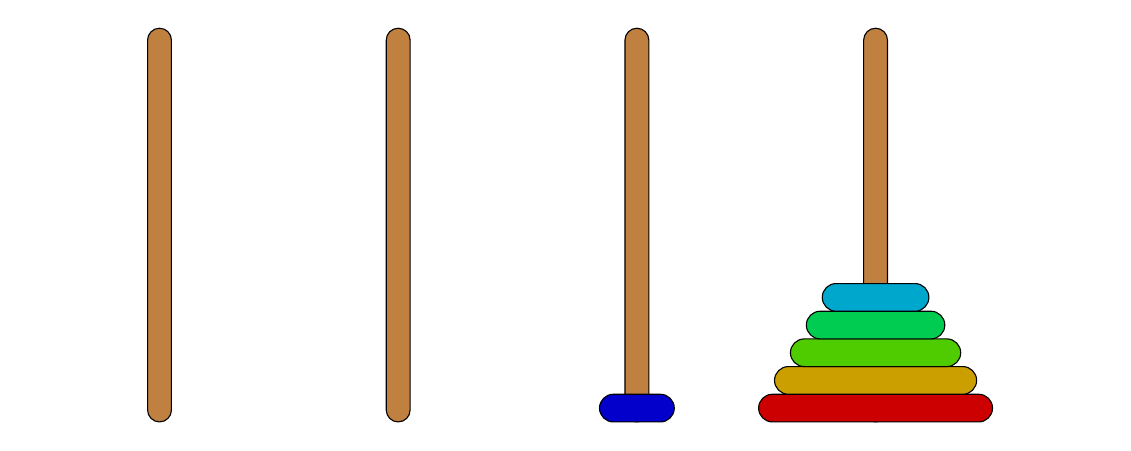
\begin{tikzpicture}
\pgfmathsetlengthmacro\diskheight{10};
\pgfmathsetmacro\k{4};
\pgfmathsetlengthmacro\step{\textwidth/\k};
\draw[color = white] (\step/2,0) -- (\textwidth+\step,0);
\foreach \n in {1,...,\k} \draw [fill = brown, draw = black, rounded corners = \step/20] (\step*\n,0) rectangle (\step*\n+\step/10,5);
\definecolor{mycolor}{rgb:hsb}{0.67,1,0.8}
\draw [fill = mycolor, draw = black, rounded corners = \diskheight/2] (\step*3+\step/20-\step*0.15666666666666668,\diskheight*0) rectangle (\step*3+\step/20+\step*0.15666666666666668,\diskheight*1);
\definecolor{mycolor}{rgb:hsb}{0.00,1,0.8}
\draw [fill = mycolor, draw = black, rounded corners = \diskheight/2] (\step*4+\step/20-\step*0.49,\diskheight*0) rectangle (\step*4+\step/20+\step*0.49,\diskheight*1);
\definecolor{mycolor}{rgb:hsb}{0.13,1,0.8}
\draw [fill = mycolor, draw = black, rounded corners = \diskheight/2] (\step*4+\step/20-\step*0.42333333333333334,\diskheight*1) rectangle (\step*4+\step/20+\step*0.42333333333333334,\diskheight*2);
\definecolor{mycolor}{rgb:hsb}{0.27,1,0.8}
\draw [fill = mycolor, draw = black, rounded corners = \diskheight/2] (\step*4+\step/20-\step*0.3566666666666667,\diskheight*2) rectangle (\step*4+\step/20+\step*0.3566666666666667,\diskheight*3);
\definecolor{mycolor}{rgb:hsb}{0.40,1,0.8}
\draw [fill = mycolor, draw = black, rounded corners = \diskheight/2] (\step*4+\step/20-\step*0.2899999999999999,\diskheight*3) rectangle (\step*4+\step/20+\step*0.2899999999999999,\diskheight*4);
\definecolor{mycolor}{rgb:hsb}{0.53,1,0.8}
\draw [fill = mycolor, draw = black, rounded corners = \diskheight/2] (\step*4+\step/20-\step*0.22333333333333333,\diskheight*4) rectangle (\step*4+\step/20+\step*0.22333333333333333,\diskheight*5);
\end{tikzpicture}
}
\only<18>{
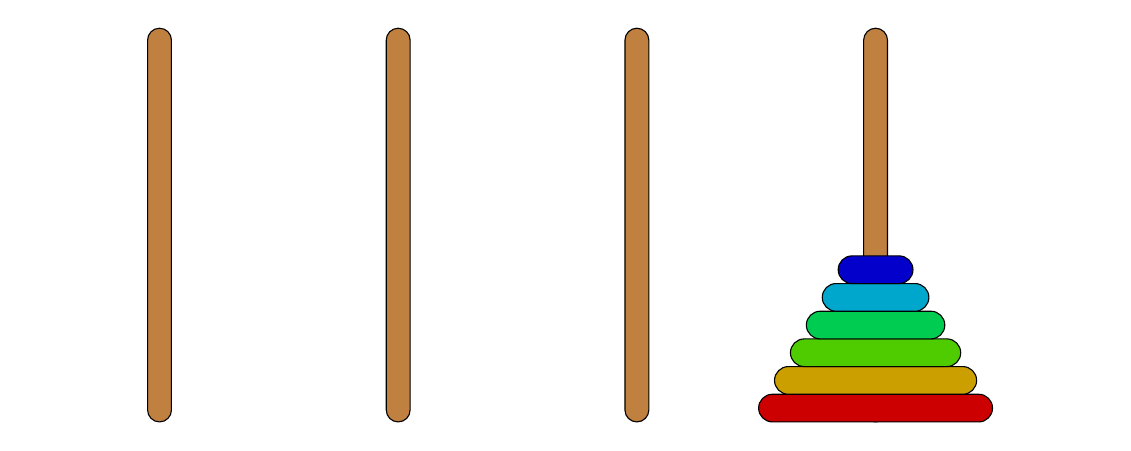
\begin{tikzpicture}
\pgfmathsetlengthmacro\diskheight{10};
\pgfmathsetmacro\k{4};
\pgfmathsetlengthmacro\step{\textwidth/\k};
\draw[color = white] (\step/2,0) -- (\textwidth+\step,0);
\foreach \n in {1,...,\k} \draw [fill = brown, draw = black, rounded corners = \step/20] (\step*\n,0) rectangle (\step*\n+\step/10,5);
\definecolor{mycolor}{rgb:hsb}{0.00,1,0.8}
\draw [fill = mycolor, draw = black, rounded corners = \diskheight/2] (\step*4+\step/20-\step*0.49,\diskheight*0) rectangle (\step*4+\step/20+\step*0.49,\diskheight*1);
\definecolor{mycolor}{rgb:hsb}{0.13,1,0.8}
\draw [fill = mycolor, draw = black, rounded corners = \diskheight/2] (\step*4+\step/20-\step*0.42333333333333334,\diskheight*1) rectangle (\step*4+\step/20+\step*0.42333333333333334,\diskheight*2);
\definecolor{mycolor}{rgb:hsb}{0.27,1,0.8}
\draw [fill = mycolor, draw = black, rounded corners = \diskheight/2] (\step*4+\step/20-\step*0.3566666666666667,\diskheight*2) rectangle (\step*4+\step/20+\step*0.3566666666666667,\diskheight*3);
\definecolor{mycolor}{rgb:hsb}{0.40,1,0.8}
\draw [fill = mycolor, draw = black, rounded corners = \diskheight/2] (\step*4+\step/20-\step*0.2899999999999999,\diskheight*3) rectangle (\step*4+\step/20+\step*0.2899999999999999,\diskheight*4);
\definecolor{mycolor}{rgb:hsb}{0.53,1,0.8}
\draw [fill = mycolor, draw = black, rounded corners = \diskheight/2] (\step*4+\step/20-\step*0.22333333333333333,\diskheight*4) rectangle (\step*4+\step/20+\step*0.22333333333333333,\diskheight*5);
\definecolor{mycolor}{rgb:hsb}{0.67,1,0.8}
\draw [fill = mycolor, draw = black, rounded corners = \diskheight/2] (\step*4+\step/20-\step*0.15666666666666668,\diskheight*5) rectangle (\step*4+\step/20+\step*0.15666666666666668,\diskheight*6);
\end{tikzpicture}
}
\end{frame}